\chapter{Características do SMI-UnB}

\section{Tecnologias Escolhidas}
Definiu-se a utilização do \textit{framework} Django \cite{django_project} como estrutura base do SMI-UnB, visto que o sistema consistiria de uma aplicação \textit{web} e que o período para desenvolvimento seria curto.

O banco de dados PostgreSQL foi escolhido como um serviço necessário para SMI-UnB, visto que o volume de informações armazenadas seria alto e que o mesmo seria capaz de atender essa demanda. Além disso, pelo Django e o PostgreSQL se tratarem de softwares livres, suas escolhas foram mais adequadas ao projeto, que por sua vez, também é livre.

    \subsection{Django}
    O Django  é um \textit{framework} para desenvolvimento \textit{web} implementado na linguagem Python\footnote{\url{https://www.python.org/}}. Sua arquitetura inspira-se no modelo tradicional MVC(\textit{Model} \textit{View} \textit{Controller}), porém, com algumas especificidades. A comunidade \textit{Django} adota o acrônimo MTV (\textit{Model} \textit{Template} \textit{View}), onde os papéis de \textit{model}, \textit{view} e \textit{controller} são redefinidos como:
    \begin{itemize}
        \item \textit{Model}: corresponde à \textit{model} do MVC tradicional e representa as classes que popularão as tabelas do banco de dados. O \textit{Django} possui um ORM (\textit{Object-Relational Mapping}, Mapeamento de Objeto Relacional) para realizar a manipulação dessas tabelas, não sendo necessário a escrita de consultas em SQL para a persistência das informações.
        \item \textit{Template}: corresponde aproximadamente à \textit{view} do MVC tradicional e descreve como as informações serão apresentadas para o usuário.
        \item \textit{View}: representada por uma função \textit{callback} referente à uma classe de URLs, descrevendo quais informações serão apresentadas e como elas serão enviadas para o \textit{template}. Alguns autores defendem que a view corresponde ao \textit{controller} do MVC tradicional, mas os próprios desenvolvedores do \textit{Django} a \textit{view} deve ser minimalista e boa parte do papel do \textit{controller} deve ser implementado nas próprias classes dos modelos.
    \end{itemize}

    Na nomenclatura do \textit{Django}, um conjunto de funcionalidades pode ser agrupado em aplicação. Cada aplicação possui suas próprias \textit{models}, \textit{views} e \textit{templates}.

    A Figura \ref{django-arq} mostra a arquitetura do \textit{Django}, apresentando as camadas do MTV durante a comunicação com o navegador até o acesso ao banco de dados. O \textit{URL dispatcher} identifica endereços requisitados pelo usuário e realiza o redirecionamento da requisição para a aplicação correta. A coordenação de requisições entre o \textit{URL dispatcher} e a \textit{view} e da \textit{view} até o \textit{template} é feita pelos chamados \textit{Middlewares}. Os \textit{Middlewares} realizam a persistência de informações entre as diferentes camadas.

    \begin{figure}[h]
        \centering
        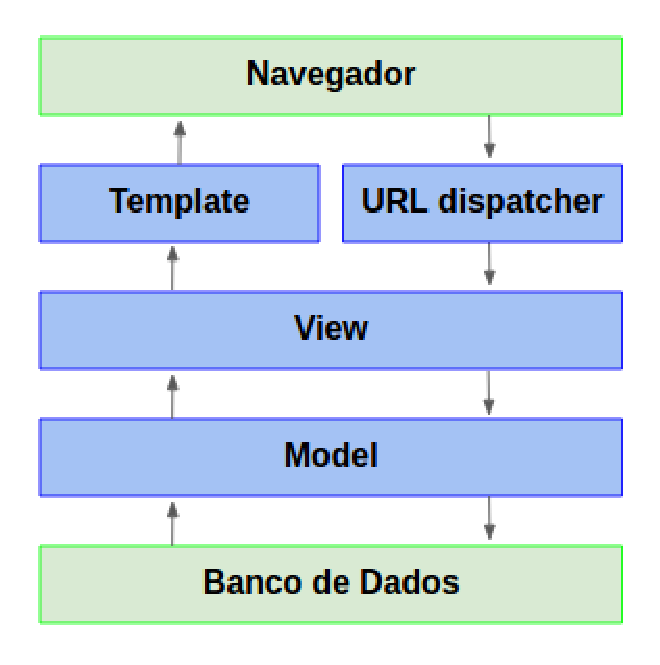
\includegraphics[keepaspectratio=true,scale=0.5]{figuras/django-arquitetura.eps}
        \caption{Arquitetura MTV \textit{Django}}
        \label{django-arq}
    \end{figure}

\section{Protocolos Utilizados}
Antes de começar o desenvolvimento, foi necessário realizar um profundo estudo sobre o equipamento para medição de dados de energia, comumente chamado de transdutor, visto que esse já havia sido pré-designado para utilização, devido a contratos realizados anteriormente pela Universidade de Brasília.

O equipamento em questão foi o TR 4020, Figura \ref{tr4020}, disponibilizado pela empresa Embrasul \cite{embrasul}. Segundo seu manual, possui frequência de amostragem a cada 50ms, comunica-se utilizando o protocolo de comunicação Modbus, no modo RTU, com velocidade de 10M/100Mbps em sistemas Ethernet utilizando o protocolo UDP como transporte. No datagrama UDP, no campo de dados, o protocolo ModBUs - RTU é encapsulado, sendo que a porta de comunicação padrão é a 1001. O endereço ModBus dos equipamentos por padrão é 1, onde a diferenciação entre equipamentos se dá pelo número de IP.

\begin{figure}[!h]
    \centering
    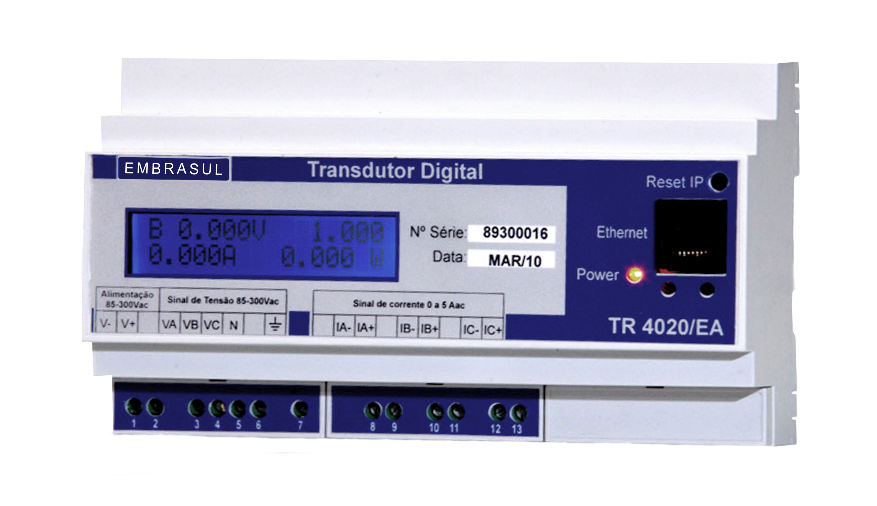
\includegraphics[keepaspectratio=true,scale=0.5]{figuras/tr4020.eps}
    \caption{Transdutor TR4020. Fonte: \cite{embrasul}}
    \label{tr4020}
\end{figure}

    \subsection{\textit{Modbus RTU}}

    \textit{Modbus} \cite{modbus} é um protocolo serial utilizado para transmitir informações entre dispositivos eletrônicos. Suas mensagens utilizam a arquitetura de mestre-escravo, como mostrado na figura \ref{mestre_escravo}. Nesta arquitetura, o papél de mestre é designado ao dispositivo que envia as requisições e escravo ao que responde passivamente às mesmas.

    \begin{figure}[!htpb]
        \centering
        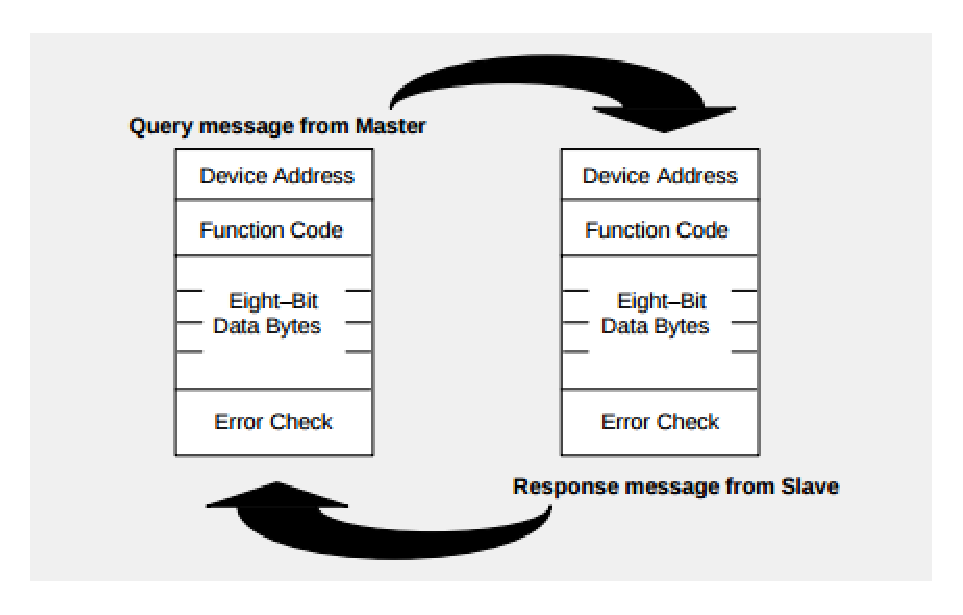
\includegraphics[keepaspectratio=true,scale=0.8]{figuras/mestre_escravo.eps}
        \caption{Comunicação Mestre-Escravo \textit{Modbus}. Fonte: \cite{modbus}}
        \label{mestre_escravo}
    \end{figure}

    Quando controladores são configurados para se comunicarem em uma rede Modbus usando o modo RTU (\textit{Remote Terminal Unit}, Unidade de Terminal Remoto) cada \textit{byte} contém duplas hexadecimais de 4 \textit{bits}. A maior vantagem de utilizar este modo é que sua grande densidade de caracteres permite uma maior taxa de transferência comparado ao modo ASCII, em uma mesma taxa de transmissão \cite{modbus}.

    Uma mensagem em Modbus RTU possui 16 \textit{bytes} e é definida da seguinte maneira:
    \begin{itemize}
        \item Identificador do Aparelho: 2 \textit{bytes}.
        \item Código de Função: 2 \textit{bytes}, define qual tipo de operação o equipamento irá realizar.
        \item Campo de Dados: 8 \textit{bytes}, sendo 4 \textit{bytes} para indicar o endereço do primeiro registrador requisitado e 4 \textit{bytes} para indicar a quantidade de registradores que serão lidos.
        \item CRC (\textit{Cyclic Redundancy Check}, Verificação de Redundância Cíclica): 4 \textit{bytes} para verificação de erros.
    \end{itemize}

    A resposta do escravo possui a seguinte estrutura:

    \begin{itemize}
        \item Identificador do Aparelho: 2 \textit{bytes}.
        \item Código de Função: 2 \textit{bytes}, define qual tipo de operação o equipamento irá realizar.
        \item Tamanho do{payload}: 2 \textit{bytes}, define o tamanho do campo de dados em \textit{bytes}.
        \item Campo de dados: possui tamanho variável, de acordo com o valor do campo anterior.
        \item CRC (\textit{Cyclic Redundancy Check}, Verificação de Redundância Cíclica): 4 \textit{bytes} para verificação de erros.
    \end{itemize}

    EXEMPLO DE MENSAGEM MODBUSRTU.

    \subsection{UDP}
    O protocolo UDP (\textit{User Datagram Protocol}, Protocolo de Datagrama do Usuário) é um protocolo da camada de transporte e não orientado a conexões. Seu cabeçalho, figura \ref{udp_header}, possui 8 \textit{bytes}, seguido de uma carga útil. As portas apresentadas no cabeçalho representam as máquinas de origem e destino \cite{tanenbaum_2002}.

    \begin{figure}[!htpb]
        \centering
        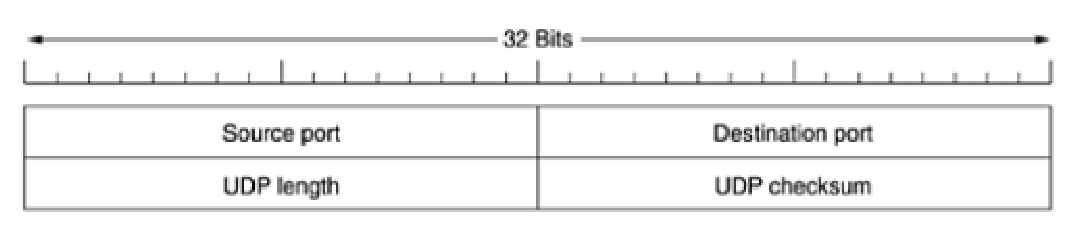
\includegraphics[keepaspectratio=true,scale=0.8]{figuras/udp_header.eps}
        \caption{Cabeçalho do UDP. Fonte: \cite{tanenbaum_2002}}
        \label{udp_header}
    \end{figure}

    Para Tanembaum, a camada de transporte é o núcleo de toda a hierarquia de protocolos. Sua função é promover uma transferência de dados confiável e econômica entre a máquina de origem e a máquina de destino, independente das redes físicas em uso no momento.

    Nas redes de acesso empresarial, uma rede de área local (LAN) é usada para conectar um sistema final a um roteador de borda. Existem muitos tipos diferentes de tecnologias LAN. No entanto, a Ethernet é a tecnologia de acesso mais prevalente nas redes corporativas. A Ethernet opera 10 Mbps ou 100Mbps e utiliza cabos par trançado para conectar uma série de sistemas finais uns com os outros e com um roteador de borda. O roteador de borda é responsável por rotear pacotes que tenham destinos fora dessa LAN. A Ethernet usa um meio compartilhado, para que os usuários finais compartilhem a taxa de transmissão da LAN \cite{kurose_2002}.

    O protocolo de camada de rede da Internet chama-se "Protocolo da Internet", ou IP. O IP fornece comunicação lógica entre hosts, possuindo um modelo de entrega de melhor esforço. Isso significa que o IP realiza seu "melhor esforço" para fornecer segmentos entre hosts comunicantes, mas não oferece garantias. Em particular, não garante a entrega do segmento, não garante a entrega ordenada de segmentos e garante a integridade dos dados nos segmentos \cite{kurose_2002}.

\section{Armazenamento das Informações}
Definiu-se que os câmpus da UnB seriam divididos por região administrativa, cada câmpus teria um conjunto de edifícios, cada edifício poderia possuir diversos transdutores e os transdutores teriam diversas medições. Para que isso fosse possível, criaram-se os \textit{apps} campuses, buildings e transductor.

No \textit{app} campuses, Figura \ref{campuses}, são definidos os modelos para uma região administrativa e os câmpus em si. A ferramenta utilizada para realizar o diagrama de classes foi a StarUML\footnote{\url{http://staruml.io/}}

\begin{figure}[!h]
    \centering
    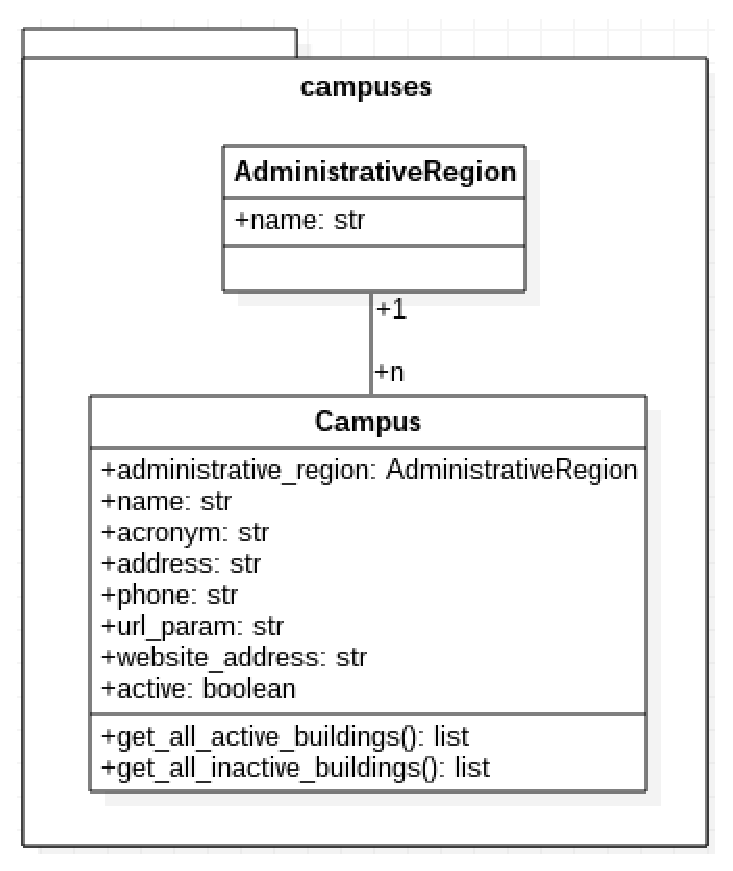
\includegraphics[keepaspectratio=true,scale=0.8]{figuras/campuses.eps}
    \caption{Diagrama de Classes para \textit{app} campuses.}
    \label{campuses}
\end{figure}

Seguindo o mesmo princípio, o \textit{app} buildings, Figura \ref{buildings}, define um modelo para os edifícios e possui um \textit{manager}, buscando auxiliar a manipulação de seus \textit{querysets}. Um \textit{queryset} representa uma coleção de objetos do banco de dados \cite{django_project}.

\begin{figure}[!h]
    \centering
    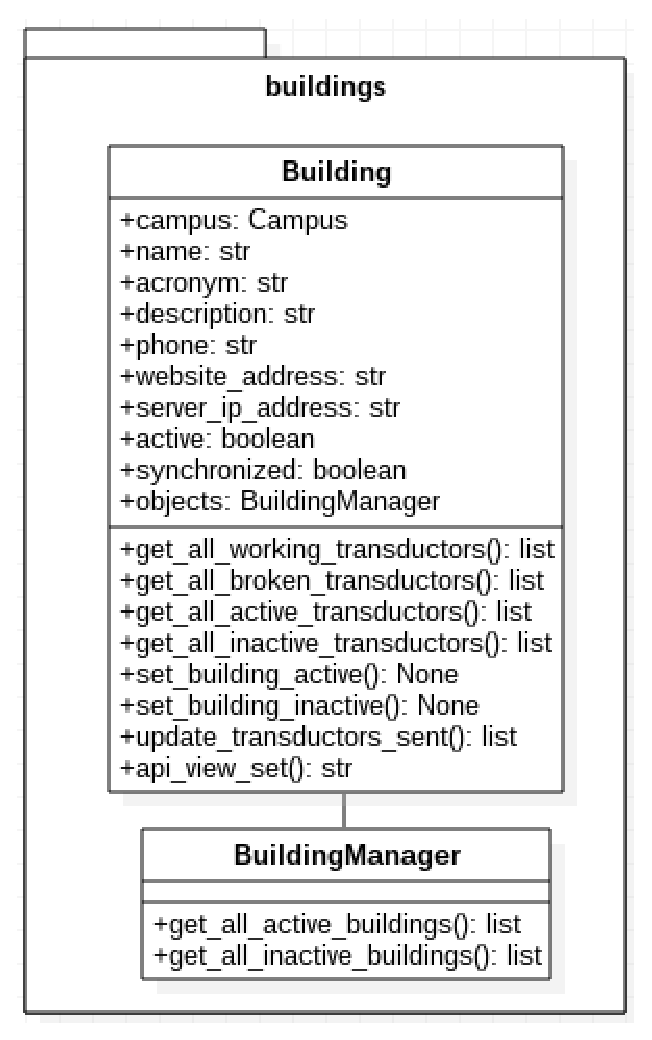
\includegraphics[keepaspectratio=true,scale=0.8]{figuras/buildings.eps}
    \caption{Diagrama de Classes para \textit{app} buildings.}
    \label{buildings}
\end{figure}

As medições de energia iriam seguir o esquema de um sistema trifásico, onde suas fases foram representadas como A, B e C. As grandezas energéticas definidas para serem coletadas foram:

\begin{itemize}
    \item Tensão.
    \item Corrente.
    \item Potência Ativa.
    \item Potência Reativa.
    \item Potência Aparente.
\end{itemize}

Os transdutores e suas medições são definidos no \textit{app} transductor, Figura \ref{transductor}. Uma das peculariedas presentes nos transdutores é a necessidade de um modelo de transdutor. Esses modelos, definidos pela classe TransductorModel, possuem toda a informação necessária para que seja possível realizar a coleta de dados, definindo o endereço e o tipo (\textit{int} ou \textit{float}) dos registradores que serão lidos, além dos protocolos seriais e de transporte utilizados.

\begin{figure}[!h]
    \centering
    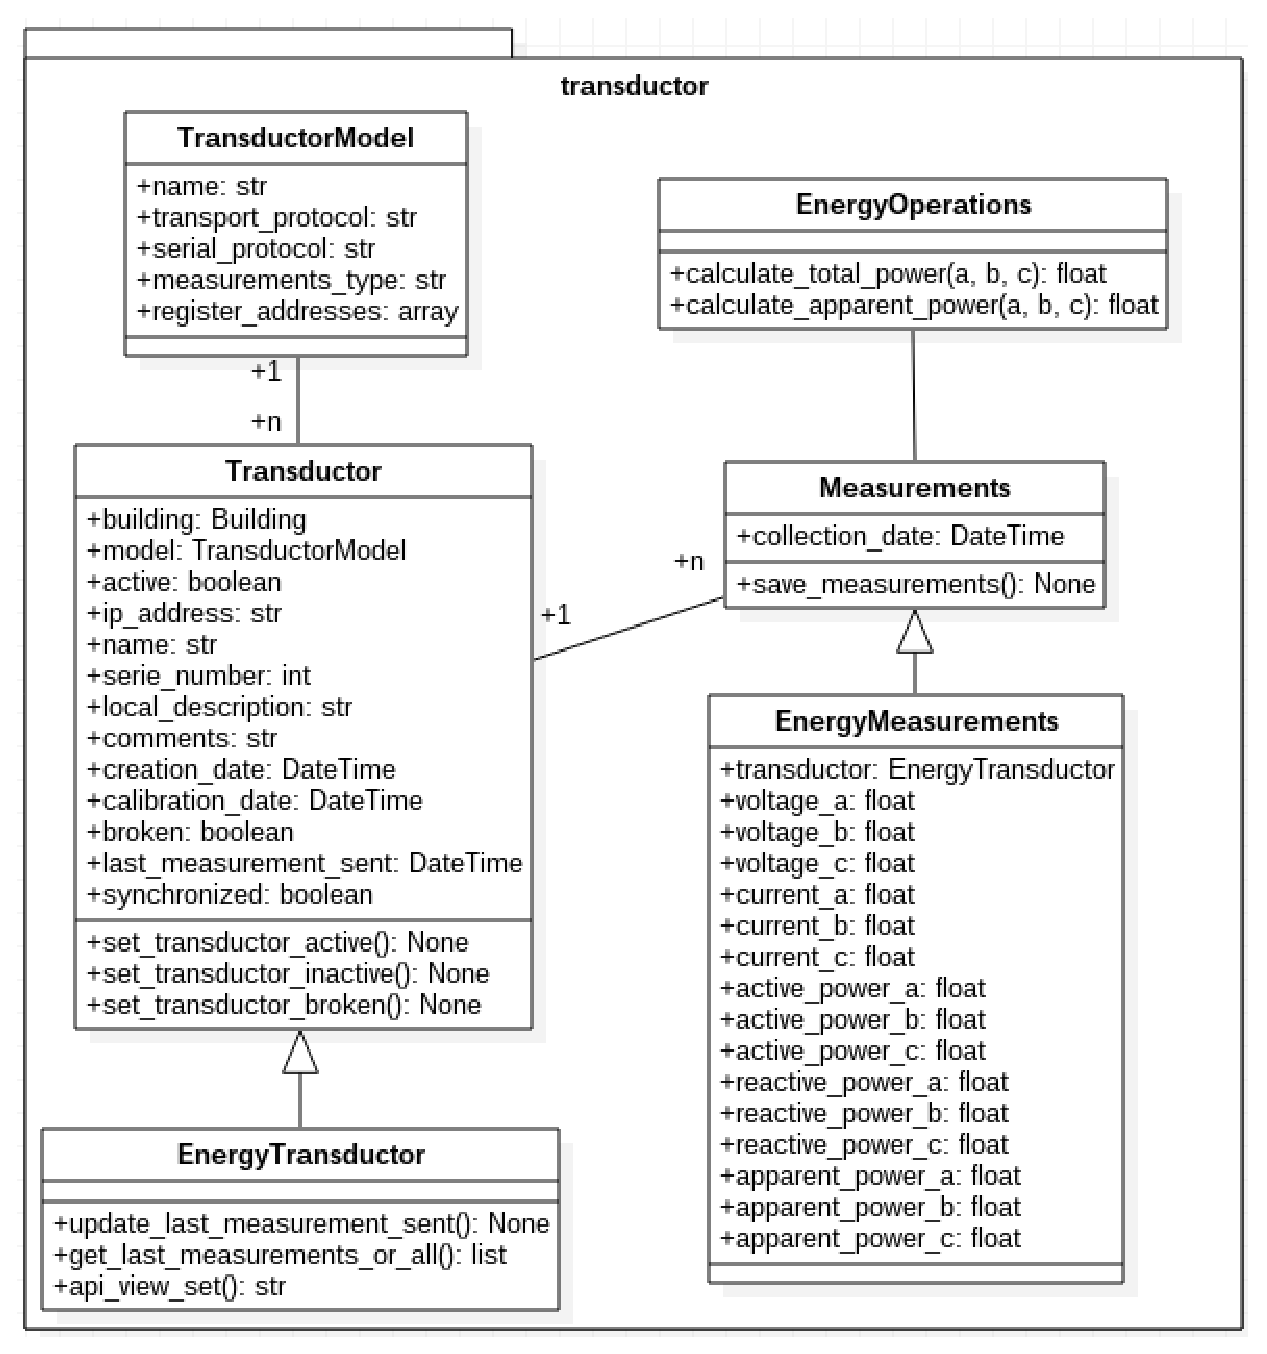
\includegraphics[keepaspectratio=true,scale=0.7]{figuras/transductor.eps}
    \caption{Diagrama de classes para \textit{app} transductor.}
    \label{transductor}
\end{figure}

As classes Transductor e Measurements são \textit{Polymorphic Models}\footnote{\url{https://django-polymorphic.readthedocs.io/en/stable/}} e possuem alguns métodos base. Com essas classes é possível extrair com mais facilidade e rapidez todas suas classes filhas, que no caso seriam as representações dos recursos monitorados pela UnB. As especializações criadas foram referentes aos transdutores de energia e medições de energia, representados pelas classes EnergyTransductor e Energymeasurements. Além disso, existe uma classe auxiliar, chamada EnergyOperations, responsável por realizar cálculos matemáticos com os dados de energia coletados.

\section{Coleta de dados}
Definiu-se que existirão dois tipos de servidores para ser possível realizar a coleta de dados inter-campi: mestre e escravo. O servidor mestre seria a representação da administração central e os escravos seriam prédios, espalhados pelos câmpus da UnB, que realizariam a coleta de dados de seus transdutores, presentes na sua mesma rede.

O tempo para coleta das informações foi definido da seguinte maneira:

\begin{itemize}
    \item A cada 1 hora, o servidor mestre seria responsável por realizar uma sincronia com todas as medições realizadas pelos escravos.
    \item A cada 1 minuto, os servidores escravos seriam responsáveis por realizarem suas coletas de dados.
\end{itemize}

\subsection{Servidor Escravo}
A coleta de dados, realizada por um prédio (servidor escravo), é feita com o auxílio do app \textit{data\_reader}, Figura \ref{data_reader}.

\begin{figure}[!h]
    \centering
    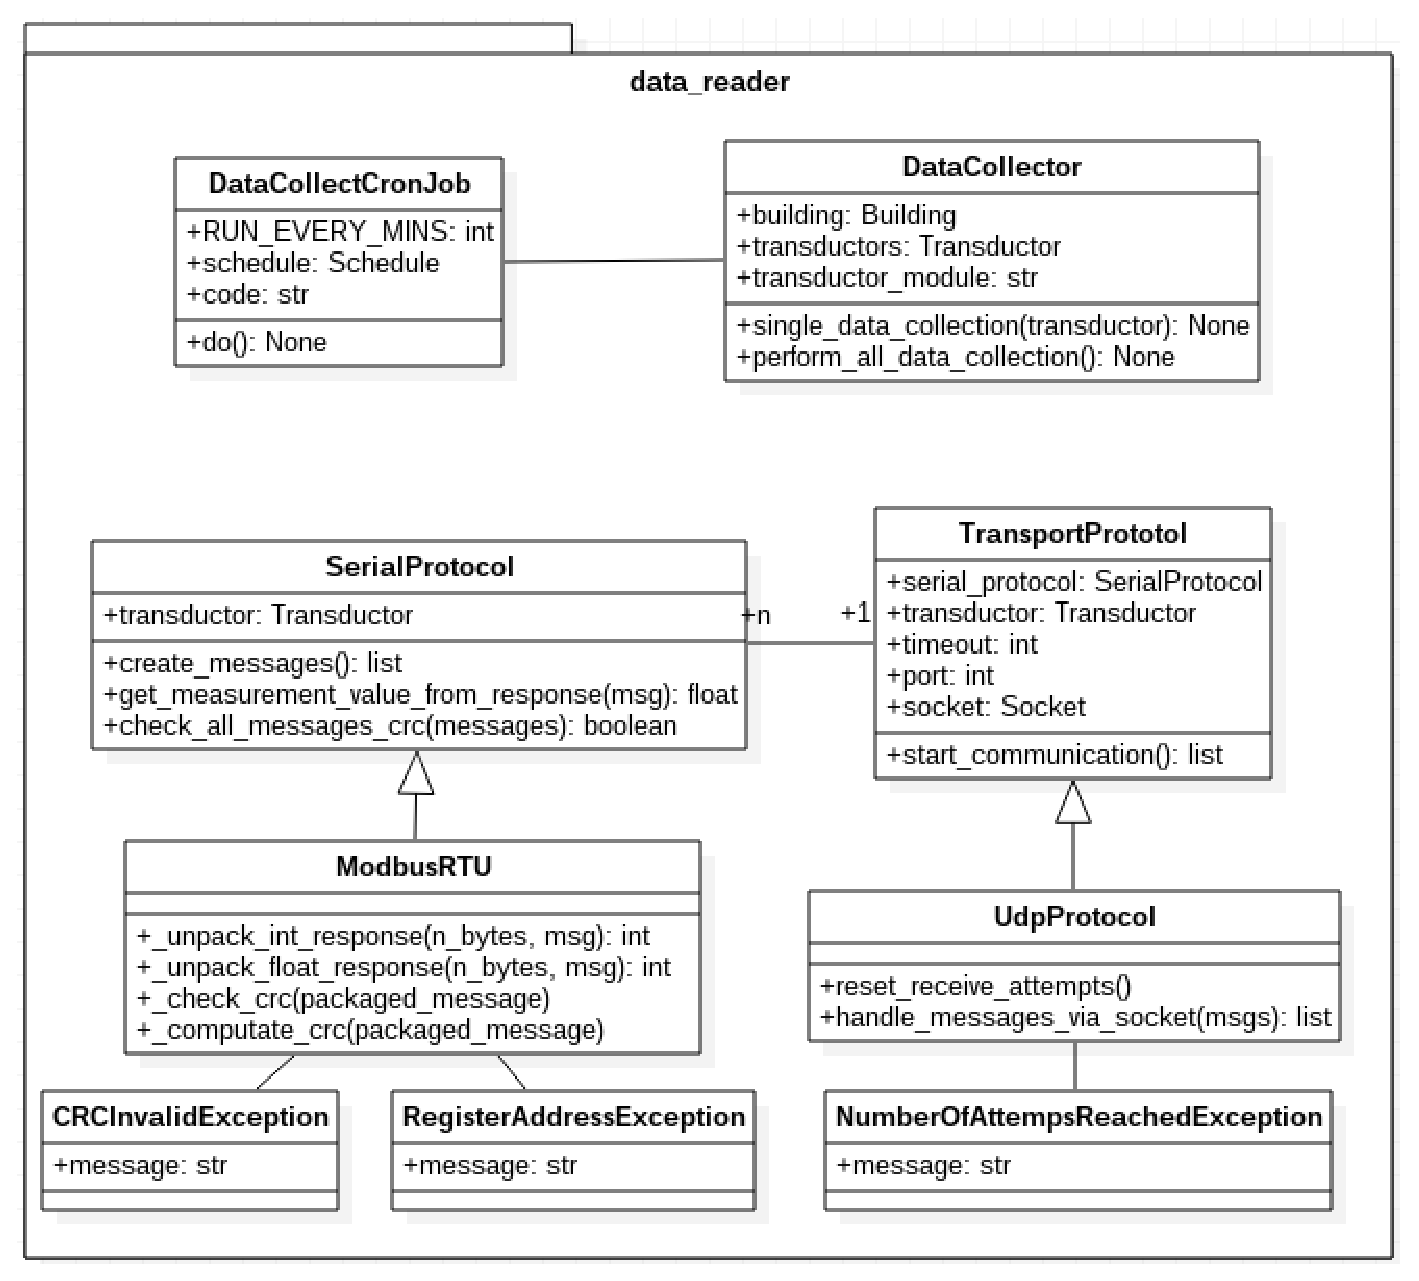
\includegraphics[keepaspectratio=true,scale=0.7]{figuras/data_reader.eps}
    \caption{Diagrama de classes para \textit{app} data\_reader.}
    \label{data_reader}
\end{figure}

A classe SerialProtocol e TransportProtocol são abstratas e possuem alguns métodos base, para que possa ser possível criar diferentes tipos de especializações, conforme a aplicação necessite. As duas, inicialmente criadas, foram referentes aos protocolos Modbus-RTU e UDP.

A coleta de dados para cada prédio, com base no equipamento TR4020, é ilustrada pela Figura \ref{process_1}. Foi utilizada a ferramenta Bizagi\footnote{\url{https://www.bizagi.com/}} para a realização da modelagem.

\begin{figure}[!h]
    \centering
    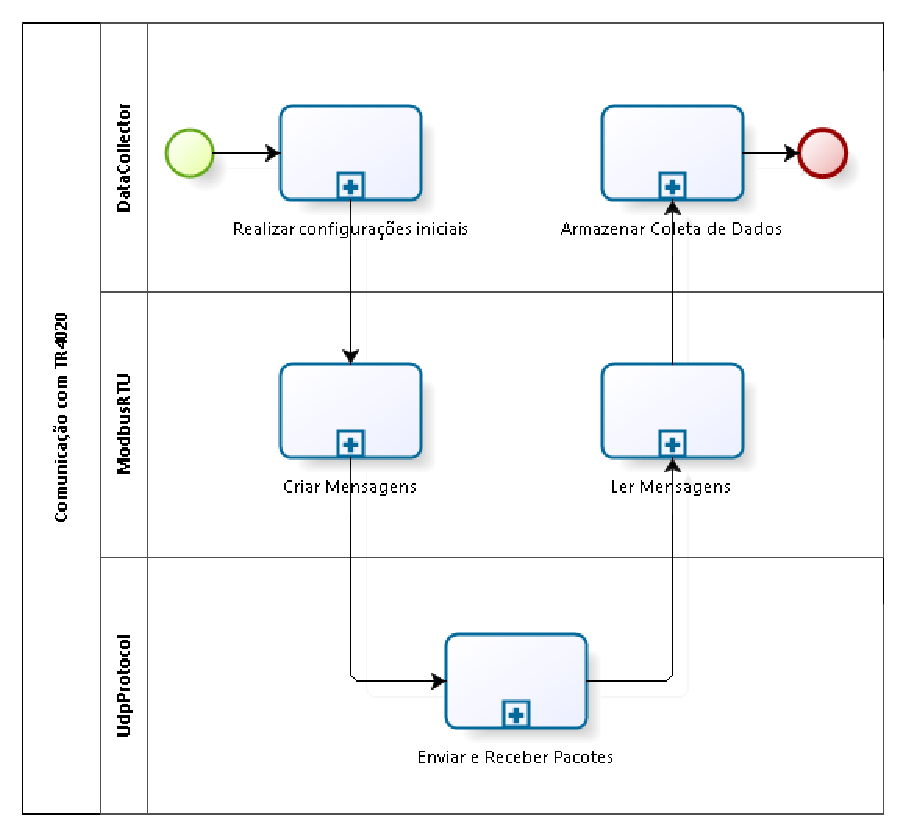
\includegraphics[keepaspectratio=true,scale=1.0]{figuras/process_1.eps}
    \caption{Coleta de dados energéticos utilizando TR4020.}
    \label{process_1}
\end{figure}

Inicialmente, a classe DataCollector identifica todos os transdutores que estão no prédio e cria uma \textit{thread} para cada um, objetivando paralelismo na coleta de dados. Segundo Tanembaum \cite{tanenbaum_2007}, as \textit{threads} são entidades escalonadas para a execução sobre a CPU, permitindo que múltiplas execuções ocorram no mesmo ambiente de um processo, com um grande grau de independência uma da outra.

Em cada \textit{thread} é identificado o modelo TR4020 para o transdutor, o qual possui as informações sobre os protocolos Modbus-RTU e UDP. A classe ModbusRTU prepara todas as mensagens que deverão ser lidas pelo equipamento, uma para cada grandeza energética e para cada fase. As mensagens seriais criadas são recebidas pela classe UdpProtocol, que irá tentar realizar a comunicação com o aparelho. Os pacotes são enviados e recebidos, um por um, até que todos sejam recebidos corretamente. Com os pacotes recebidos, são extraídas suas cargas úteis, que basicamente correspondem às medições de cada grandeza, logo após, as mesmas são lidas, utilizando a classe ModbusRTU. Por fim, a classe DataCollector recebe as medições e as salva.

A coleta temporizada, a cada 1 minuto, das medições energéticas realizadas pelos prédios é realizada pela ferramenta \textit{cron} \cite{paul_cron}, presente em sistemas UNIX. O \textit{cron} é \textit{daemon} para executar comandos de agendamento. Um \textit{daemon} é programa que é executado em segundo plano e visa estar sempre em execução, caso seja iniciado. Além disso, o \textit{cron} utiliza o \textit{crontab} para manter os arquivos, que possuem instruções a serem executadas periodicamente, de cada usuário. Um arquivo mantido pelo \textit{crontab} deve seguir a estrutura do Algoritmo \ref{crontab}

\begin{python}[caption={Estrutura de um arquivo mantido pelo \textit{crontab}.}, captionpos=b, label={crontab}]
minuto hora dia_mes mes dia_semana comando_para_execucao
# Linha em banco para deixar cron valido
\end{python}

Adicionou-se um novo comando para aplicação, chamado \textit{runcrons}. Esse comando é definido pela ferramenta django-cron\footnote{\url{http://django-cron.readthedocs.io/en/latest/}} e basicamente executa um código que possua como base a classe \textit{CronJobBase}. Esse código, após ser executado, é bloqueado até que o tempo de espera para outra execução seja atingido, como uma espécie de cronômetro.

Criou-se a classe DataCollectCronJob, Algoritmo \ref{data_collect}, objetivando invocar o DataCollector para realizar a coleta de dados. O arquivo mantido pelo crontab para realizar a coleta, periodicamente a cada 1 minuto, foi definido conforme o Algoritmo \ref{cron_slave}.

\begin{python}[caption={Classe DataCollectCronJob.}, captionpos=b, label={data_collect}]
class DataCollectCronJob(CronJobBase):
    RUN_EVERY_MINS = 0
    schedule = Schedule(run_every_mins=RUN_EVERY_MINS)
    code = 'smi_unb.data_reader.cronjob.DataCollectCronJob'

    def do(self):
        data_collector = DataCollector()
        data_collector.perform_all_data_collection()
\end{python}

\begin{python}[caption={\textit{Cron} para execução da coleta dos dados de energia.}, captionpos=b, label={cron_slave}]
* * * * * python3 /SMI-UnB/manage.py runcrons \
smi_unb.data_reader.cronjob.DataCollectCronJob
# Necessary line at end of file to make cron valid
\end{python}

\subsection{Servidor Mestre}
O servidor mestre não realiza nenhuma coleta de dados, sendo esse responsável por realizar uma sincronização com os dados coletados pelos servidores escravos por meio de uma API \textit{web}.

\textit{Application Programming Interface} (API) é um conjunto de requisitos que regem como um aplicativo pode conversar com outro. As APIs realizam isso expondo algumas das funções internas de um programa para o mundo exterior de forma limitada, possibilitando que os aplicativos compartilhem dados e tomem ações em nome do outro, sem exigir que os desenvolvedores compartilhem todo o código do software \cite{brian_api}.

Quando usado no contexto do desenvolvimento \textit{web}, uma API é tipicamente definida como um conjunto de requisições do protocolo HTTP, juntamente com uma definição da estrutura de mensagens de resposta, geralmente utilizando as linguagens \textit{Extensible Markup Language} (XML) ou \textit{JavaScript Object Notation} (JSON) \cite{benslimane_2008}.

O \textit{Hypertext Transfer Protocol} (HTTP), é um protocolo \textit{web} presente na camada de aplicação do modelo OSI e é implementado por dois programas: um cliente e outro servidor. Os programas cliente e servidor conversam entre si, trocando mensagens HTTP, sendo que o protocolo define como o cliente (por exemplo, um navegador) solicitará páginas \textit{web} de um servidor (por exemplo, o Django) e como o servidor irá transferir essas páginas para o cliente \cite{kurose_2002}.

A API utilizada no projeto baseou-se no Django REST Framework \cite{django_rest}. O \textit{Representational State Transfer} (REST) \cite{fielding_2000} é um estilo arquitetural para projetar sistemas distribuídos e apresenta as seguintes características:

\begin{itemize}
    \item Estado e funcionalidade são divididos em recursos distribuídos.
    \item Todo recurso é exclusivamente endereçável, usando um conjunto uniforme e mínimo de comandos.
    \item O protocolo é cliente/servidor, sem estado, em camadas e suporta armazenamento em \textit{cache}.
\end{itemize}

O Django REST Framework utiliza alguns métodos HTTP para mapear as operações CRUD (criar, resgatar, atualizar e deletar) nas requisições HTTP, sendo esses:

\begin{itemize}
    \item GET: recuperar informações de uma entidade.
    \item POST: criar ou atualizar uma entidade.
    \item PUT: criar ou atualizar uma entidade. O método PUT é idempotente, ou seja, se uma operação for realizada duas vezes sobre o mesmo objetivo, não haverá efeito.
    \item PATCH: modificar parcialmente uma entidade.
    \item DELETE: deletar uma entidade.
\end{itemize}

O conceito de \textit{endpoints} é utilizado pelo Django REST Framework, objetivando a interação com a API do lado do servidor, pois especificam onde os recursos podem ser acessados, por meio da classe padrão ModelViewSet.

A sincronia de dados é realizada pela classe EnergyMeasurementSynchronizer, presente no \textit{app} \textit{api}, Figura \ref{api}. Em linhas gerais, essa classe realiza duas requisições HTTP para cada servidor escravo. Na primeira requisição são consumidas as medições de energia mais recentes de cada transdutor, via API. Com as medições resgatadas, atualiza-se o horário da última coleta de dados de cada transdutor, no servidor mestre. Após atualizados os horários no mestre, realiza-se a segunda requisição, que atualiza o horário de todos os transdutores presentes no escravo.

\begin{figure}[!h]
    \centering
    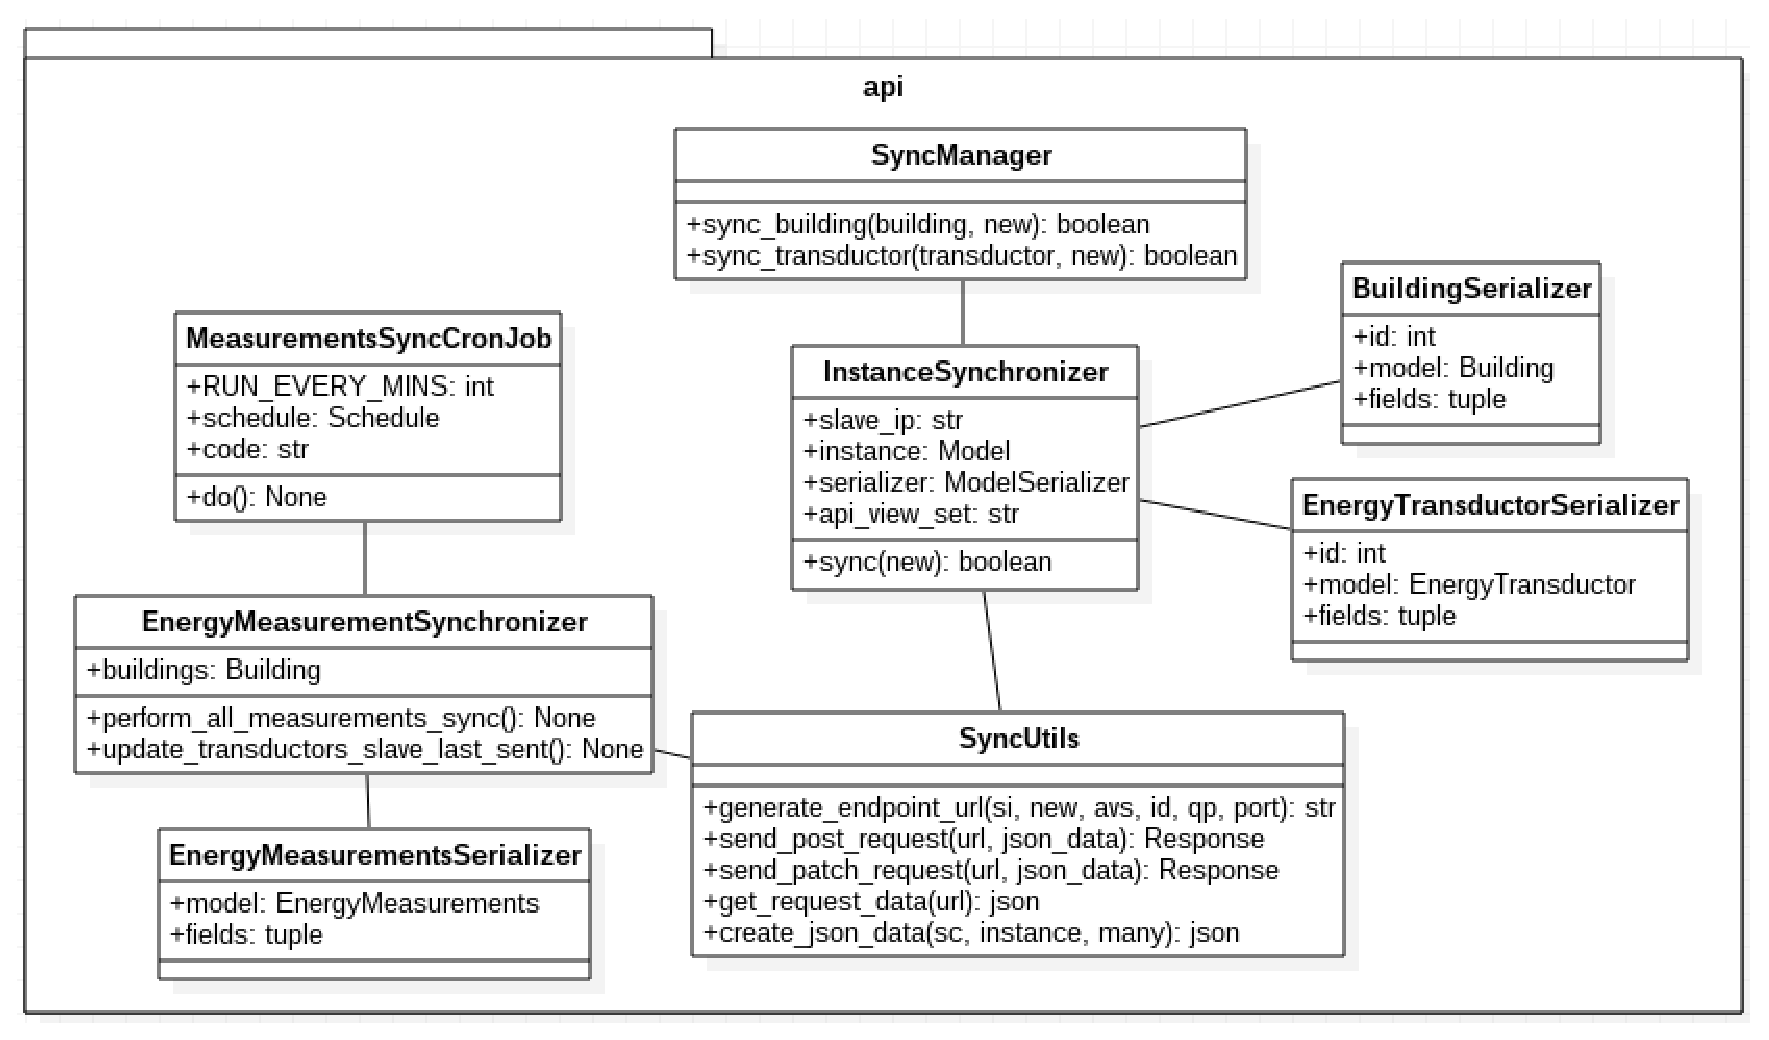
\includegraphics[keepaspectratio=true,scale=0.55]{figuras/api.eps}
    \caption{Diagrama de classes para \textit{app} api.}
    \label{api}
\end{figure}

O \textit{cron} para se realizar a sincronia das medições, a cada 1 hora, é expresso pelo Algoritmo \ref{cron_master} e utiliza a classe MeasurementsSyncCronJob, Algoritmo \ref{measu_sync}.

\begin{python}[caption={\textit{Cron} para execução da sincronia dos dados de energia.}, captionpos=b, label={cron_master}]
0 * * * * python3 /SMI-UnB/manage.py runcrons \
smi_unb.api.cronjob.MeasurementsSyncCronJob
# Necessary line at end of file to make cron valid
\end{python}

\begin{python}[caption={Classe MeasurementsSyncCronJob.}, captionpos=b, label={measu_sync}]
class MeasurementsSyncCronJob(CronJobBase):
    RUN_EVERY_MINS = 59
    schedule = Schedule(run_every_mins=RUN_EVERY_MINS)
    code = 'smi_unb.api.cronjob.MeasurementsSyncCronJob'

    def do(self):
        e_synchronizer = EnergyMeasurementSynchronizer()
        e_synchronizer.perform_all_measurements_sync()
\end{python}

\section{Segurança}
Realizou-se um sistema de login por meio de email, para facilitar os usuários na hora de se autenticarem no sistema. O django já possui um módulo de autenticação bem definido, que realiza tanto a autenticação quanto a autorização de um usuário. Como esse módulo realizava login por meio do nome de usuário, algumas mudanças foram implementadas para ser possível o login por meio de email. Para isso, criou-se o \textit{app} authentication, Figura \ref{authentication}, o qual define a classe EmailBackend, que por sua vez realiza a autenticação por email.

\begin{figure}[!h]
    \centering
    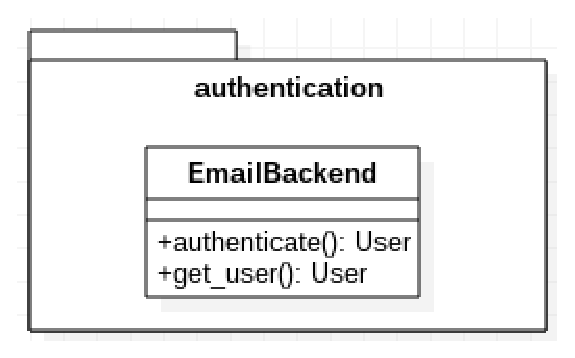
\includegraphics[keepaspectratio=true,scale=0.8]{figuras/authentication.eps}
    \caption{\textit{App} authentication}
    \label{authentication}
\end{figure}

Vale ressaltar que o Django realiza. TERMINAR TEXTO sobre segurana de passwords no django.

\begin{python}[caption={Corpo do método authenticate, classe EmailBackend.}, captionpos=b]
class EmailBackend(ModelBackend):
    def authenticate(self, username=None, password=None, **kwargs):
        UserModel = get_user_model()
        try:
            user = UserModel.objects.get(email=username)
        except UserModel.DoesNotExist:
            return None
        else:
            if getattr(
                user, 'is_active', False
            ) and user.check_password(password):
                return user
        return None
\end{python}

Os transdutores e prédios presentes no sistema não podem ser excluídos, tendo em vista a importância de se deixar registrado suas medições realizadas. Para isso acontecer, alguns botões de habilitar e desabilitar foram adicionados à aplicação e um atributo referente a ativo foi adicionado aos seus modelos.

Sincronia

O servidor mestre é responsável por realizar todo o registro/edição de transdutores e prédios. Assim, sempre que se tenta realizar uma operação desse tipo, o mestre tenta comunicar-se com o escravo, por meio de uma requisição HTTP, utilizando o método GET. Vale ressaltar que esta solução ainda deve ser aperfeiçoada, buscando aceitar, também, requisições Https.

\begin{python}[caption={Corpo do método is\_valid, classe EnergyForm.}, captionpos=b]
class EnergyForm(forms.ModelForm):
    ...

    def is_valid(self):
        ...

        url = 'http://' + self.instance.building.server_ip_address
        try:
            request = requests.get(url, timeout=3)
        except:
            self.add_error(
                None,
                _('Unable to communicate with Building server.')
            )
            return False
\end{python}

Definiram-se, inicialmente, duas permissões para os usuários: gerencia de prédios e de transdutores. Cada uma dessas permite ao usuário os direitos de incluir, modificar e habilitar/desabilitar. A gerência de usuários e definição das permissões são realizadas pelo \textit{app} users, Figura \ref{app_users}.

\begin{figure}[!h]
    \centering
    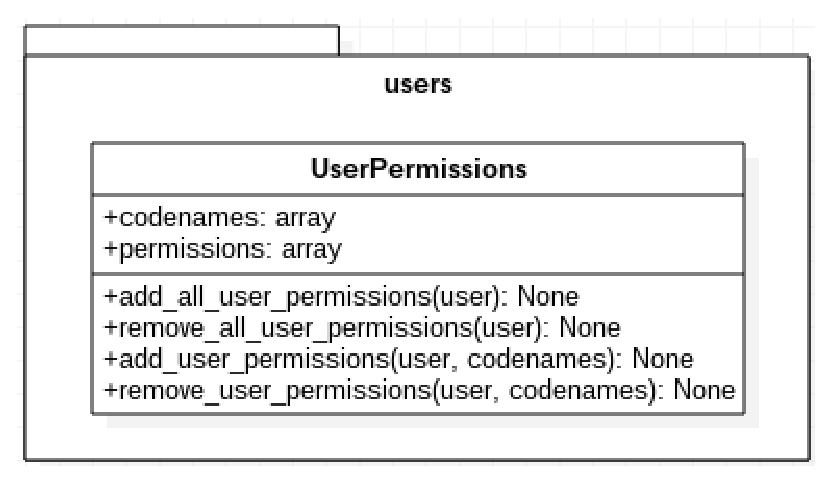
\includegraphics[keepaspectratio=true,scale=0.8]{figuras/app_users.eps}
    \caption{Diagrama de classes para \textit{App} users.}
    \label{app_users}
\end{figure}

\begin{python}[caption={Permissões presentes na classe UserPermissions.}, captionpos=b]
class UserPermissions(models.Model):
    ...

    class Meta:
        permissions = (
            ("manager_buildings", "Manager Buildings"),
            ("manager_transductors", "Manager Transductors"),
        )
\end{python}

Secret key gerada automaticamente

\section{Gerência de Configuração}
Utilizou-se o Docker \cite{docker} para que fosse possível criar um ambiente unificado para o sistema, visando evitar futuros problemas de implantação.

O Docker é uma plataforma de contêiners de software. Um contêiner, Figura \ref{container}, possui empacotado tudo que é necessário para se executar um software completo ou parte dele. Diferente das máquinas virtuais, os contêiners são executados em uma mesma máquina, compartilhando o kernel do seu sistema operacional, sendo que cada um terá seu processo isolado no espaço de usuário.

\begin{figure}[!h]
    \centering
    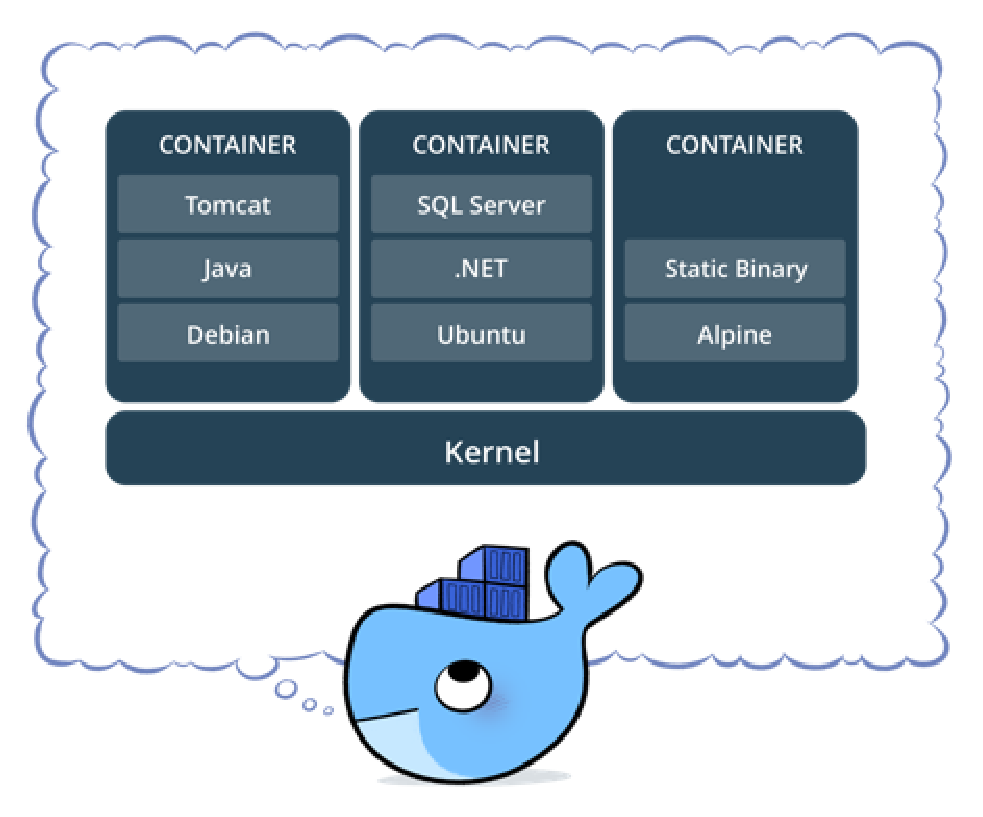
\includegraphics[keepaspectratio=true,scale=0.8]{figuras/container.eps}
    \caption{Exemplo de contêiners providos pelo Docker. Fonte: \cite{docker} }
    \label{container}
\end{figure}

Para Tanenbaum \cite{tanenbaum_2007}, o sistema operacional é a peça mais básica de software e opera em modo núcleo, possuindo acesso completo a todo o hardware e ao conjunto de instruções oferecidos pela máquina. O resto do software opera em modo usuário, onde é disponível para execução apenas um conjunto de instruções da máquina.

Criaram-se duas configurações para os ambientes referêntes ao mestre e escravo, onde suas diferenciações baseavam-se basicamente no cron que seria executado em cada um. Para realizar essas configurações utilizou-se a ferramenta Docker Compose, tornando mais fácil a definição e execução de múltiplos contêiners. Os serviços definidos para a aplicação foram:

Linkar os containers.

\begin{itemize}
    \item nginx: fornecimento dos arquivos estáticos.
    \item web: fornecimento da aplicação em Django.
    \item postgres: armazenamento das informações.
    \item redis: \textit{cache} da aplicação.
    \item data: armazenamento do banco de dados.
\end{itemize}

O serviço nginx

Http

WSGI

O script de integração contínua do projeto, Figura \ref{integracao}, utiliza imagens oficiais do Python 3.5 e do Postgresql, presentes no Docker-Hub\footnote{\url{https://hub.docker.com/}}, que é repositório oficial de imagens do Docker. Todas as imagens do docker-hub já estão prontas para serem executadas em contêiners. Após os contêiners serem iniciados e vinculados, é realizada a instalação dos pacotes utilizados pelo SMI-UnB. Com a instação dos pacotes, inicia-se verificação das normas da PEP8, com a ferramenta flake8 e por fim, são executados todos os testes do sistema e exibida a cobertura total, por meio da ferramenta Coverage\footnote{\url{https://pypi.python.org/pypi/coverage/}}.

\begin{figure}[!h]
    \centering
    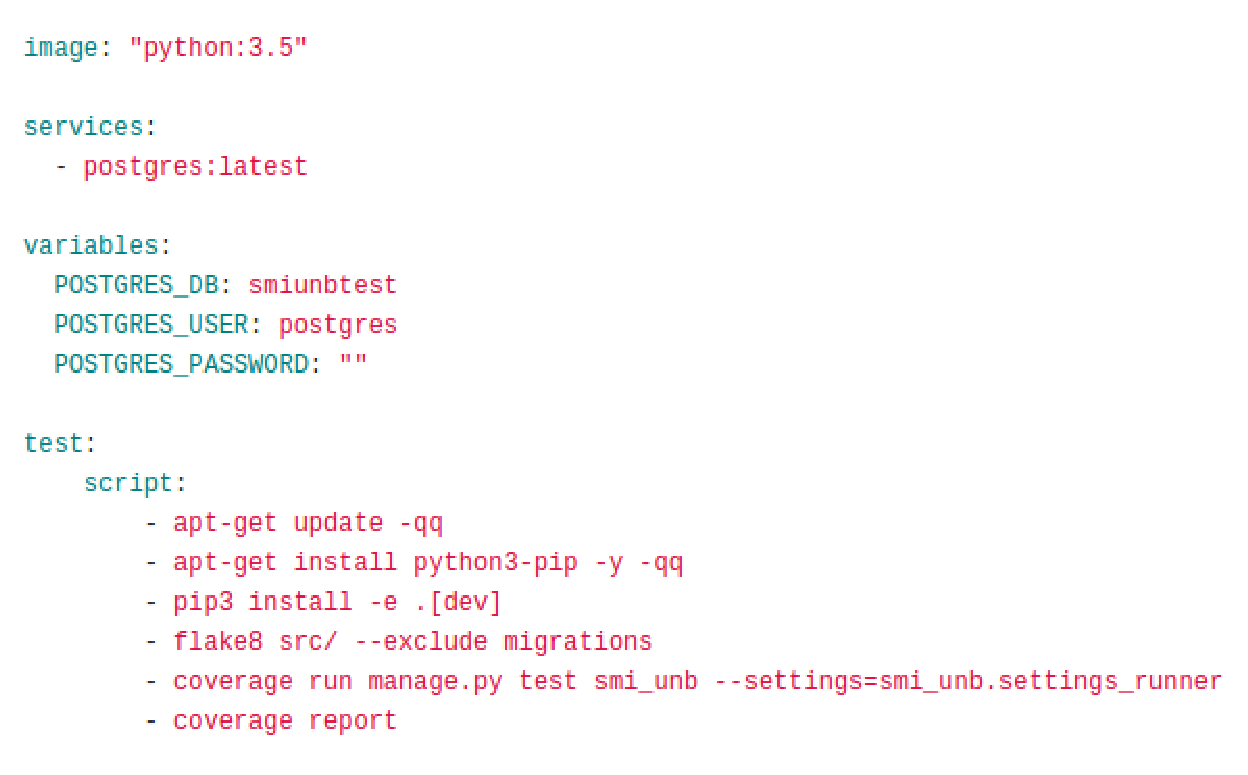
\includegraphics[keepaspectratio=true,scale=0.65]{figuras/integracao.eps}
    \caption{\textit{Script} para integração contínua do projeto.}
    \label{integracao}
\end{figure}

Tasks

Fixtures

\section{Apresentação das Informações}
O \textit{framework} Bootstrap foi utilizado como base para se realizar o \textit{layout} da aplicação, por possuir estruturas bem definidas e fáceis de serem utilizadas. Os ícones utilizados foram provenientes do Font Awesome\footnote{\url{http://fontawesome.io/}}. Tanto o Boostrap quanto o Font Awesome são disponilizados sobre uma licença livre e podem ser utilizados em qualquer projeto, contanto que haja uma referêcia sobre os mesmos.

Javascripts usados

Imagens da aplicação
\section{Métricas}
Codeclimate

sloccount

\section{Visão Geral do Sistema}
    \subsection{Diagrama de Classes por \textit{App}}
    Interessante para quem quer entender o sistema (Software livre)

    Apresentar diagrama
    \subsection{Testes}
    Testes unitários com Mock

    Cobertura
    \section{Requisitos Mínimos}
    Rodar linux

    Rede?
